../cictikz/src/cictikz/data/tex/cictikz_preamble.tex

% Well proximity effect: during the well implant, ions scatter off the
% photoresist edge and land in the silicon nearby, so devices close to
% the well edge see higher doping and a higher threshold voltage.

\definecolor{echarge}{RGB}{30,60,220}
\definecolor{hcharge}{RGB}{220,30,30}
\definecolor{implant}{RGB}{40,150,60}

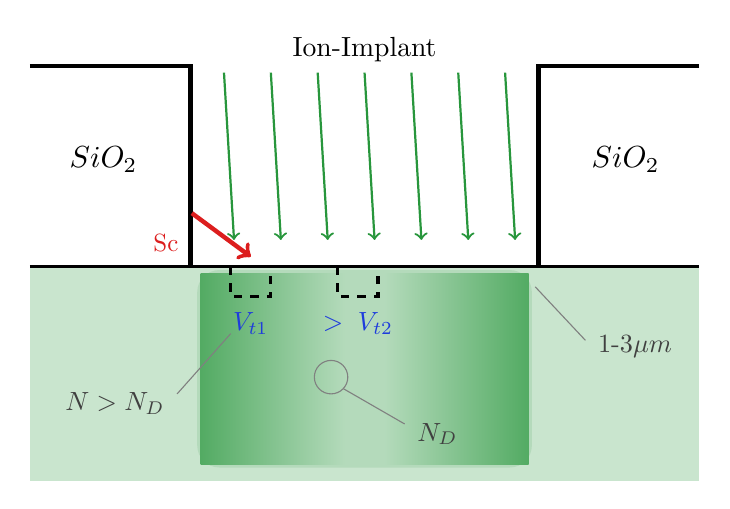
\begin{tikzpicture}[scale=0.85]

  % photoresist masses
  \draw[line width=1.6pt] (0.0,5.6) -- (2.4,5.6) -- (2.4,2.6);
  \draw[line width=1.6pt] (10.0,5.6) -- (7.6,5.6) -- (7.6,2.6);
  \node[anchor=center, scale=1.1] at (1.1,4.2) {$SiO_2$};
  \node[anchor=center, scale=1.1] at (8.9,4.2) {$SiO_2$};

  % silicon with the implanted well. The shading is the doping: the
  % scattered ions pile up against both resist edges, so the well is
  % darkest there and fades to the nominal N_D in the middle.
  \fill[implant!25] (0.0,2.6) rectangle (10.0,-0.6);
  \fill[implant!35, rounded corners=8pt] (2.5,2.55) rectangle (7.5,-0.4);
  \shade[left color=implant!80, right color=implant!35] (2.55,2.5) rectangle (4.7,-0.35);
  \shade[left color=implant!35, right color=implant!80] (5.3,2.5) rectangle (7.45,-0.35);
  \draw[line width=1.2pt] (0.0,2.6) -- (10.0,2.6);

  % the implant rain
  \foreach \x in {2.9,3.6,...,7.3}{
    \draw[implant, thick, ->] (\x,5.5) -- (\x+0.15,3.0);
  }
  \node[anchor=center, scale=1.0] at (5.0,5.85) {Ion-Implant};

  % the scattered ion off the resist edge
  \draw[hcharge, line width=1.6pt, ->] (2.42,3.4) -- (3.3,2.75);
  \node[hcharge, anchor=east, scale=0.9] at (2.35,2.95) {Sc};

  % two identical transistors, different distance to the well edge
  \draw[line width=1.2pt, dashed] (3.0,2.6) rectangle (3.6,2.15);
  \draw[line width=1.2pt, dashed] (4.6,2.6) rectangle (5.2,2.15);
  \node[echarge, anchor=north, scale=0.95] at (3.3,2.05) {$V_{t1}$};
  \node[echarge, anchor=north, scale=0.95] at (4.9,2.05) {$>\; V_{t2}$};

  % doping annotations
  \draw[thin, gray] (3.0,1.6) -- (2.2,0.7);
  \node[anchor=east, scale=0.95, gray!50!black] at (2.15,0.55) {$N > N_D$};
  \draw[thin, gray] (4.5,0.95) circle (0.25);
  \draw[thin, gray] (4.68,0.78) -- (5.6,0.25);
  \node[anchor=west, scale=0.95, gray!50!black] at (5.65,0.1) {$N_D$};

  % distance from the well edge that matters
  \draw[thin, gray] (7.55,2.3) -- (8.3,1.5);
  \node[anchor=west, scale=0.95, gray!50!black] at (8.35,1.4) {1-3$\mu m$};

\end{tikzpicture}
\end{document}
